\chapter{Infrastructure Provisioning}  
\label{chapter:infrastructure-provisioning}
    In this chapter we will take a look at the core question of how the infrastructure necessary for realizing the reference architecture from \autoref{chapter:architecture-proposal} can be provisioned. Since provisioning managed cloud services is a solved problem, this chapter will focus on provisioning on bare-metal machines while taking into account that a uniform strategy for provisioning the infrastructure of all environments (edge, fog and cloud) should be chosen.

    \section{Advantages and Challenges in Bare-Metal Infrastructure}

    In IIoT systems having own hardware is almost always a non-negotiable factor, especially when it comes to edge computing (see \autoref{section:edge-computing}), which is why thinking about bare-metal infrastructure is inevitable in IIoT systems. Before taking a look at solutions for bare-metal infrastructure provisioning, we must first look at why bare-metal is such a challenge in the first place. The layering of abstractions is a recurring strategy in the history of computing. However, building abstractions over bare-metal machines is still a central problem that needs to be addressed, since physical machines are the fundamental pieces that underlie everything in the software ecosystem. The need for properly configured and managed hardware that is solid and capable of fulfilling today's requirements regarding load, stress, strain and even external influences like fire, earthquakes or a pandemic is higher than ever. The main issue regarding building a solid abstraction over bare-metal nowadays is the lack of standardization in APIs for provisioning and management. APIs that exist, OpenStack being the most common one, are often extremely complex and impose huge amounts of operational effort \cite{building_future_on_metal}. Other than that, maintaining bare-metal infrastructure has several other drawbacks. These include the high effort and complexity, the necessity for dedicated specialists, higher initial cost and lower flexibility and scalability compared to cloud resources. Once the machines are provisioned, the lack of services managed by cloud providers like object storage, virtual networks or databases poses another challenge. \newline

    Using bare-metal infrastructure also brings several beneficial factors however. First of all, it makes use cases like edge computing and low-latency applications possible, which are common requirements in IIoT. Owning hardware can also be more cost-effective compared to utilizing cloud provider resources, especially after the initial investment (buying hardware, engineering cost for abstractions, etc.) is amortized. This is especially noticeable in performance efficiency, since the full computational power of the hardware is available, compared to cloud-managed machines which often experience overhead due to virtualization. Furthermore, bare-metal machines offer higher standards when it comes to security, isolation and compliance as there is more control over both physical and network access. Moreover, while resources are shared among multiple tenants in a cloud system, which can lead to fluctuations in performance (``noisy neighbor problem''), bare-metal machines provide dedicated resources and thus offer more predictable performance. Custom hardware also performs better for workloads that are not fit for virtualized environments like database servers or GPU-heavy workloads for machine learning. Lastly, having open solutions built upon own hardware results in no dependence on a cloud provider thus minimizing the risk of a vendor lock-in \cite{building_future_on_metal}.

    
    \section{Provisioning Kubernetes}
\label{section:bare-metal-provisioning}
    In \autoref{chapter:architecture-proposal} we introduced a reference architecture that revolves around Kubernetes as its central technology. This section will deal with strategies that will allow us to provision Kubernetes on a wide variety of infrastructure ranging from physical hardware in the edge and fog environments up to cloud providers in the cloud environment. To understand this section in its entirety, a basic understanding of Kubernetes is required.

    
    \subsection{Required Infrastructure}
    \label{subsection:provisioning}
    As mentioned earlier, while having own bare-metal machines imposes many benefits, it comes at the cost of having to manage the machines across their full lifecycle. This begins with provisioning the machines, which typically means to perform tasks like
    
    \begin{itemize}
        \item picking a suitable server from a pool of available servers
        \item applying specific configuration for hardware (like network interfaces or RAID controllers) and low-level software (like firmware or BIOS)
        \item loading appropriate software (operating system, drivers, applications) as well as user data into it
        \item applying necessary updates to minimize vulnerabilities in software
        \item configuring network stack, monitoring, applications, etc.\ \cite{building_future_on_metal}
    \end{itemize}

    \noindent In order to achieve this, we once again aim to find a uniform solution that not only works for bare-metal machines but for all environments of the proposed reference architecture from \autoref{chapter:architecture-proposal}. The solution should also have domain knowledge regarding our central technology Kubernetes and its operational tasks like provisioning and upgrading. Lastly, the solution should work in a declarative manner in order to be compatible with our GitOps setup. \newline
    
    Let us take a look at what we need to provision infrastructure-wise in order to be able to implement the reference architecture. As already mentioned above the basis for any bare-metal machine is configuring the hardware and installing the necessary software, which at least includes an operating system (OS), ideally one that is optimized for hosting containerized applications (see \autoref{subsection:containers-and-os}). With the OS installed, the system must now be configured for production readiness regarding the hosting of Kubernetes. This includes network configuration, disabling swap memory, configuring the kernel and the firewall and many more configurations domain-specific to Kubernetes. The system is now ready for the installation of Kubernetes. On top of Kubernetes, a network plugin and a storage plugin must be chosen and installed depending on the infrastructure that K8s runs upon.

    This setup is simpler for the cloud environment since most cloud providers offer managed instances of Kubernetes (Azure Kubernetes Service, Amazon EKS, Google Kubernetes Engine, etc.) out of the box. If managed virtual machines are chosen, the steps of the previous paragraph, starting with configuring the OS, apply. Once the environments are all running Kubernetes, a GitOps controller (see \autoref{section:gitops}) needs to be deployed in each Kubernetes instance and configured to reconcile the according desired state from Git. From then on, all deployments, configurations, etc.\ can be done through GitOps by adding changes to Git.\newline
    
    Since we seem to encounter different types of scenarios regarding infrastructure we will explore these briefly. The easiest scenario is provisioning managed Kubernetes within a cloud provider, which is a solved problem and can be done with a variety of tools. The next scenario are servers, both bare-metal or virtual in the cloud, that already have an operating system provisioned, which can be handled by using remote connection protocols like SSH or standard IT automation tools. Similar to that are scenarios where a virtualization platform (see \autoref{section:virtualization}) like VMware vSphere is used since these often provide sane APIs to create virtual machines, which brings us back to the scenarios that were already mentioned. The last scenario is having to provision bare-metal machines which is also the most challenging due to the lack of tooling and standardization. 

    \subsection{Technical Solutions and Tooling}
    
    Let us now explore potential technical solutions (i.e.\ tooling) that are capable of provisioning and managing infrastructure in all of these scenarios. For such tasks, IT automation tools like Ansible, Chef or Puppet quickly come to mind. With these, it is easy to automate tasks like provisioning Kubernetes onto machines or a managed Kubernetes instance of a cloud provider. In the real bare-metal world, these tools however are often infeasible to use, since they expect machines to already be provisioned with an operating system which often is not the case. To tackle this challenge, we could provision an operating system by network booting the machine using technologies like ``PXE Boot'' and ``IPMI'' (see \autoref{subsection:network-boot}) and then use an automation tool like Ansible. However, there are even more shortcomings with such tools. Configuration automation tools mostly operate on a push-based approach. This method lacks continuous reconciliation and monitoring capabilities, which are e.g.\ essential for automatically provisioning new hardware without manual intervention, for taking action in case of hardware or software failures or in general detecting and handling a drift between the desired and actual state. They are also not Kubernetes-aware, which makes operational tasks like upgrading Kubernetes more demanding.

    Another strategy following the principle of immutable infrastructure, where components are replaced rather than changed or updated in place, would be to install a prebuilt OS image via network boot. This OS image could already contain everything required for running a production-ready instance of Kubernetes (see \autoref{subsection:provisioning}) and would require no further modifications after booting. This method is similar to the previous one, but also lacks continuous reconciliation and an understanding of Kubernetes, making it unviable for large-scale systems. It also introduces a serious security risk, since the OS image would also contain sensitive information like the Kubernetes join token. Consequently, anyone who gains access to this image could potentially join the Kubernetes cluster, posing a substantial vulnerability. Also, the use of a manually started network boot prevents us from fully committing to the GitOps framework.

    An ideal solution that fulfills all requirements is the project "ClusterAPI", which we will explore in detail in the following section.
    

    \subsection{ClusterAPI}
    \label{subsection:capi}

    Let's consult the official description provided by the developers of ClusterAPI (CAPI) to understand how they characterize the project:

    \begin{quote}
        ``Cluster API is a Kubernetes subproject focused on providing declarative APIs and tooling to simplify provisioning, upgrading, and operating multiple Kubernetes clusters. Started by the Kubernetes Special Interest Group (SIG) Cluster Lifecycle, the Cluster API project uses Kubernetes-style APIs and patterns to automate cluster lifecycle management for platform operators. [...] This enables consistent and repeatable cluster deployments across a wide variety of infrastructure environments.'' -- ClusterAPI, GitHub \cite{capi_github}
    \end{quote}

    \noindent This description gives us a great overview of the project. It offers a standardized solution for the challenge of managing and operating Kubernetes clusters throughout their lifecycle at scale by abstracting the underlying complexity. Note that the Kubernetes SIG is also the maintainer of well-known projects like ``kOps'' and even ``kubeadm'', both of which offer tooling for creating production-ready Kubernetes clusters. \newline

    ClusterAPI is a Kubernetes-native project and consists mainly of custom Kubernetes Operators, which are software extensions to Kubernetes that make use of custom resources to manage applications and their components \cite{k8s_operator_pattern}. The operators run instances of so-called custom controllers, which are responsible for the continuous reconciliation of the custom resources like ``Cluster'' or ``Machine''. In this process, each controller continuously watches for drift between the desired and the actual state described in these custom resources and takes according actions when a drift is detected. Since these custom objects are nothing but Kubernetes manifests (i.e.\ YAML files) we can store them in Git, thus providing a great integration into our GitOps (see \autoref{section:gitops}) setup. When using ClusterAPI, a separate Kubernetes cluster is used as a ``Management Cluster''. This cluster is mainly responsible for managing the lifecycle of the so-called ``Workload Clusters''. It can also host common infrastructure like central observability (see \autoref{section:observability}) or a multicluster management solution (see \autoref{section:multicluster-mgmt}) but must not be used for running domain-specific workloads \cite{efficient_k8s_capi}.\newline

    Let us now take a look at how ClusterAPI can solve all of the different provisioning scenarios mentioned in \autoref{subsection:provisioning} that we typically find in the real world. The project achieves this by providing flexible extensibility through a provider system, which in practice behaves similarly to a plugin design. The documentation states, that ``Cluster API can be extended to support any infrastructure (AWS, Azure, vSphere, etc.), bootstrap or control plane (kubeadm is built-in) provider'' \cite{capi_github}.

    \begin{figure}[htbp]
        \centering
        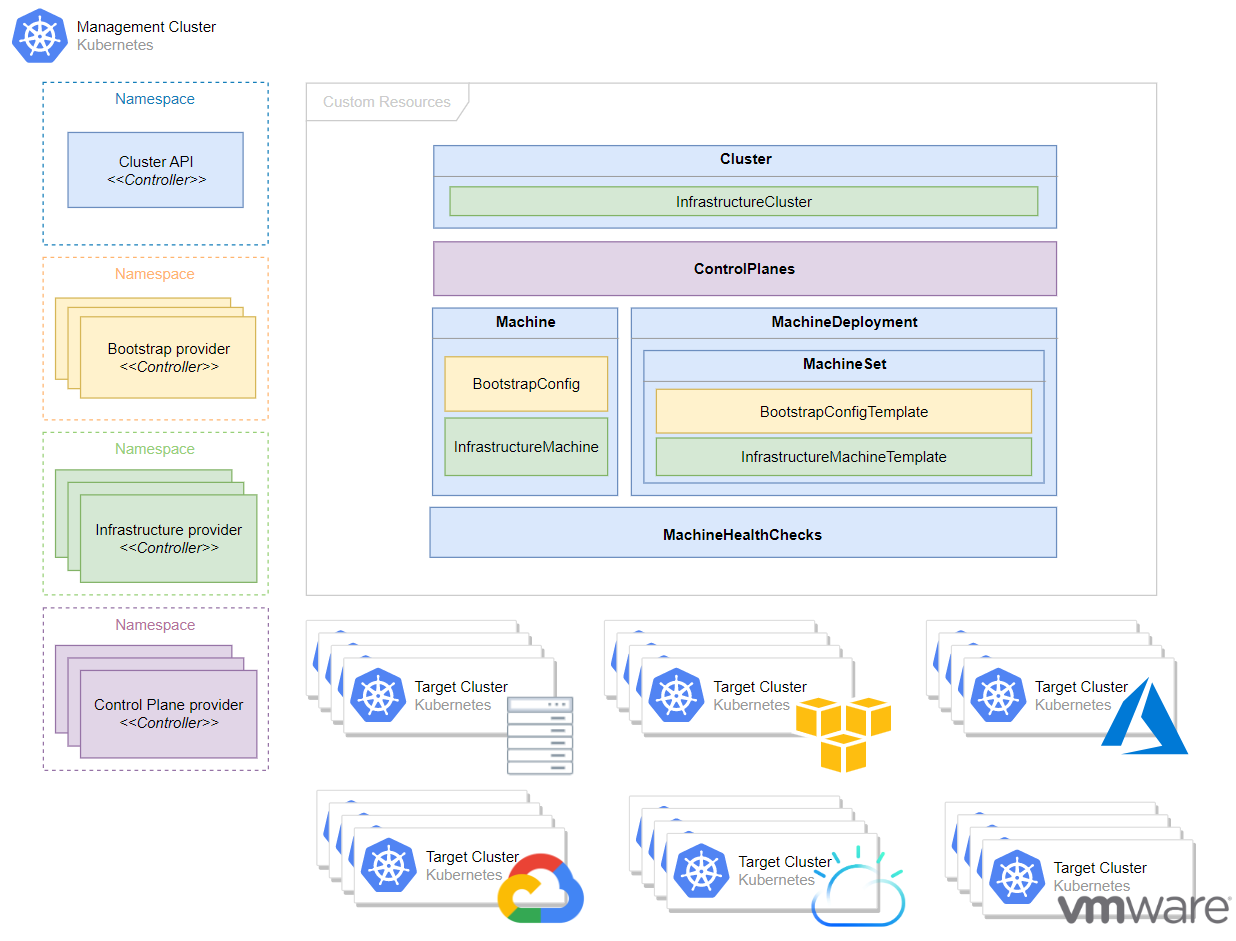
\includegraphics[width=0.9\textwidth]{img/capi.png}
        \caption{ClusterAPI Concepts \cite{the_cluster_api_book}}
        \label{figure:capi}
    \end{figure}

    \noindent \autoref{figure:capi} shows the architecture that makes this high degree of extensibility possible. The top right section shows components and custom resource definitions that ClusterAPI ships by default. These can be seen as the most generic components that basically provide interfaces for provider-specific components to implement as we will see later. 
    
    The most important custom resource definitions for this work are the ``Cluster'', ``ControlPlane'' and ``Machine''-resources. The ``Cluster'' resource is a resource that is responsible for grouping all other related resources to managed Kubernetes clusters and is the most abstract of them all. Within the cluster, we can see an ``InfrastructureCluster'', which in practice is a reference to a specific cluster resource from an ``Infrastructure provider''. Below that we see the ``ControlPlanes'' which again is a high-level abstraction over a Kubernetes control plane. In practice, the according ``Control Plane provider'' specific control plane resource is located within the cluster resource as a reference. Lastly, the ``Machine'' custom resource definition is a ``declarative spec for an infrastructure component hosting a Kubernetes Node'' \cite{the_cluster_api_book}. We observe two instances of provider-specific references in each machine object: one is related to a resource from the ``Bootstrap provider'', and the other to a resource of the ``Infrastructure provider'' \cite{spectrocloud_2022}. All of these providers are explained further in the next paragraph. From the perspective of ClusterAPI, all ``Machine'' objects are immutable: once they are created, they are never updated, only deleted. For this reason, so-called ``MachineDeployments``, which are similar to Kubernetes Deployments, are preferable and used in practice rather than using ``Machine'' objects directly \cite{the_cluster_api_book}. The other components in this section of \autoref{figure:capi} are not relevant for this work. It is hence up to the reader to explore these independently, according to their interest or need.\newline

    Since we saw that the ClusterAPI resources are mostly high-level abstractions that include references to provider-specific implementations, we must now understand what these providers are responsible for. The providers allow developers to provision workload clusters on their desired infrastructure and abstract away all necessary interaction with the actual infrastructure, ranging from on-premises bare-metal systems up to cloud providers \cite{efficient_k8s_capi}. The ability to create infrastructure that can be maintained, destroyed and re-deployed with little human interaction embodies the philosophy of treating servers as ``cattle, not pets'', ensuring that systems are easily manageable, rather than being treated as irreplaceable individual entities. This is the dream in the environment of physical hardware since it offers interaction with the infrastructure that feels very similar to using a cloud provider \cite{cattle_not_pets}.

    For this interaction, the ``Infrastructure provider'' holds all responsibility. Depending on the provider it has the capabilities necessary to provision managed resources in the cloud, virtual machines in a virtualization platform or even physical bare-metal machines that are required by other ClusterAPI objects. The ``Bootstrap provider'' on the other hand is responsible for turning a provisioned machine into a Kubernetes node, which is typically done using cloud-init. This mainly involves creating the necessary configuration to bootstrap the Kubernetes control plane and worker nodes, generating cluster certificates and joining nodes to the cluster. The ``Control Plane provider'' is very similar since it is responsible for building and reconciling the configuration for the Kubernetes control plane nodes. Through references the provider-specific resources are mapped in a one-to-one relationship where one ClusterAPI resource refers to one specific provider resource and vice versa \cite{the_cluster_api_book, spectrocloud_2022}.\newpage

    \noindent Using this flexibility we can now provision Kubernetes clusters in all infrastructure scenarios discovered in \autoref{subsection:provisioning}: cloud providers, virtualization platforms and bare-metal machines both with and without an operating system installed just by choosing the appropriate providers. In \autoref{chapter:poc} we will provision a managed cluster in the Microsoft Azure cloud and a bare-metal cluster onto a physical machine using such providers. Overall ClusterAPI is a proven solution for managing Kubernetes clusters that fits this use case perfectly. Companies like Mercedes-Benz use ClusterAPI to manage hundreds to thousands of Kubernetes clusters in production which further validates the use of CAPI \cite{mercedes_kubecon_700}. Another validating example is ``Gardener'' which is a common tool for managing the full lifecycle of conformant Kubernetes clusters as a service. The documentation states that the project, while not using it directly, is heavily inspired by ClusterAPI and still follows it with great interest to this day \cite{gardener_capi}. Similarly, the popular multicluster management platform ``Rancher'' by SUSE leverages ClusterAPI under the hood for provisioning their Kubernetes distribution RKE2 \cite{rancher_uses_clusterapi}.
    
    \subsection{Out-of-Band Management and Network-Based Boot}
    \label{subsection:network-boot}

    While we have found a tool that is capable of uniformly managing Kubernetes-based infrastructure across all environments in our systems with ClusterAPI, we still have not taken a look at how ClusterAPI provisions and manages physical servers, which is the actual challenge when dealing with bare-metal machines. While the previous section only explained this with the use of a provider/plugin system, this section will deal with the technical details. \newline

    \subsubsection{Out-of-Band Management}
    \label{subsubsection:oob-management}
    
    The centerpiece of any proper bare-metal management solution is a microcontroller called baseboard management controller (BMC) within the hardware, which makes it possible to remotely manage and monitor hardware independent of its operating system or status, even when it is powered off. The ability to perform such operations is often referred to as ``Integrated Lights out Management'' (ILOM) or ``Out-of-Band Management'' (OoB) \cite{was_ist_bmc}. These operational features are exposed for external access via the network by an interface, the most common one being the IPMI (Infrastructure Platform Management Interface). Note that all of this depends on the hardware and is only possible if a BMC is available.

    The interface was first released in 1998 and was developed by Intel, Hewlett-Packard, Dell and NEC with the goal of making remote management of servers possible - even when they are powered off or have no operating system installed. Using this interface to access the BMC, operators can for example monitor sensor data of the system and install software, drivers or updates. The most important feature in the context of this work however is the ability to power the machine on or off remotely \cite{was_ist_ipmi_datacenter}. This feature allows for remotely powering machines on or off, enabling them to be booted up by ClusterAPI infrastructure providers as needed, thereby preparing the machine for the subsequent steps of provisioning.

    \subsubsection{Network Boot}
    Once the system is booting, an operating system needs to be provisioned. Typically, ClusterAPI infrastructure providers designed for bare-metal machines will choose a Kubernetes optimized OS like Flatcar Linux, Fedora CoreOS or Talos Linux as described in \autoref{subsection:containers-and-os}. In order to achieve full automation during the OS installation, most ClusterAPI providers rely on the strategy of booting the machines via the network. One of the most popular models for this is the Preboot Execution Environment (PXE) which we will briefly discuss in this work. \newline

    The client-server model PXE which was originally developed by Intel is an open industry standard that enables network-capable machines, which are referred to as PXE clients, to boot via a server in the local network. The process requires a machine with a PXE-enabled network interface card (i.e. the PXE client), a custom configuration in the network's DHCP server and a TFTP server.\newline

    \begin{figure}[htbp]
        \centering
        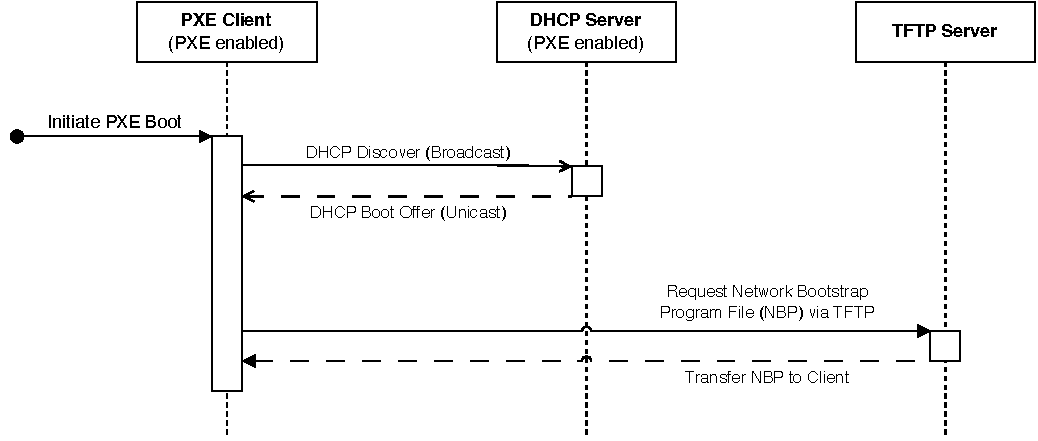
\includegraphics[width=0.9\textwidth]{img/pxe-boot.pdf}
        \caption{PXE Boot Process}
        \label{figure:pxe-boot}
    \end{figure}

    \noindent \autoref{figure:pxe-boot} shows the steps of a network boot using PXE. The PXE-Client initiates the process by sending a standard DHCP discover packet with PXE-specific boot parameters and system information set as a broadcast into the local network. A DHCP-Server that supports PXE and is configured properly will reply to the network boot request broadcast with the necessary information to perform a network boot, whereas other DHCP-Servers will simply ignore the flag and continue with the standard four-way DHCP handshake. This implies that setting up additional DHCP servers in the network, specifically dedicated to handling boot requests, is practical. These additional servers are commonly referred to as ``Proxy DHCP-Servers''. This approach allows for the separation of boot request management from IP address allocation or just using PXE even though the pre-existing DHCP server does not support it. If the PXE/DHCP server is in a separate network, which causes DHCP broadcasts to not reach their intended target destination, many routers offer a functionality in the form of a router rule called ``ip helper'', which configures the router to forward these packets to their according target in the according network. \newline 
    
    \noindent The response (boot offer) from the PXE-enabled DHCP server contains two necessary DHCP options that have to be configured in the DHCP server in advance: 

    \begin{itemize}
        \item Option 66 (TFTP Server Name): Hostname or IP address of the TFTP server
        \item Option 67 (Boot File Name): Path of the boot file on the TFTP server
    \end{itemize}

    \noindent The last step for the PXE client is to reach out to the TFTP server (DHCP Option 66) and download the boot file (DHCP Option 67) from it into memory via the TFTP protocol. This boot file is also referred to as the network bootstrap program (NBP) and has the task of preparing the client for running the specified operating system. The client boots using this NBP, which typically leads to the download and finally the launch of the actual operating system \cite{paragon_software_pc_deployment}. Similar to what was described regarding out-of-bands management in the previous \autoref{subsubsection:oob-management}, ClusterAPI infrastructure providers specialized towards bare-metal infrastructure will typically either ship their own or have integrations with external DHCP and TFTP servers. Once the operating system is running, ClusterAPI can continue to provision Kubernetes as described in \autoref{subsection:capi}. Note that this was a concise overview of the PXE boot process. For more detailed information, readers are encouraged to further explore the topic.

    \subsubsection{Shortcomings of PXE and IPMI}
    While PXE and IPMI are very common solutions, they are both old and no longer up-to-date to today's standards and will be replaced by more modern successors like HTTP Boot for PXE and Redfish for IPMI eventually. \newline

    PXE has a major issue regarding security since it offers no mechanism for encryption or authentication natively, which makes the standard vulnerable to attacks like a man-in-the-middle attack using a rogue DHCP server that hands out malicious boot information. Since no authentication or encryption is in place, this can hardly be prevented. Another drawback of PXE is the poor scalability due to TFTP timeouts and UDP packet loss (DHCP uses UDP). With a larger scale, these issues will occur more and more often resulting in an unreliable network boot setup. Common solutions include booting into an intermediate and more featureful network boot firmware like ``iPXE'' that from then on tackles these limitations and adds functionality like booting via HTTP or even via a wireless network whereas only LAN boots via a TFTP server are possible with plain PXE. This process is often referred to as ``chainloading''. This however imposes the use of yet another piece of software that brings complexity. The more modern approach is using HTTP Boot which acts as a replacement for PXE and tries to address these issues. HTTP Boot either uses a preconfigured or a, via DHCP, auto-discovered URL to either boot an NBP or an ISO image directly. The main difference however is its reliance on HTTP. This solves the issues of PXE regarding security by using the encrypted HTTPS protocol and the issues regarding scalability using HTTP load balancing and the more reliable TCP protocol as a layer 4 protocol base in favor of UDP \cite{pxe_ipmi_redfish_httpboot}. \newline

    Similarly to PXE, the interface for out-of-band management IPMI also has shortcomings regarding security. Not only does it lack modern security best practices, but there are also known vulnerabilities in the IPMI specification like the ``IPMI 2.0 RAKP Authentication Remote Password Hash Retrieval'' that allows remote attackers to obtain password hashes and perform offline password guessing attacks. Due to its age, IPMI struggles with modern architectures like multi-node server clusters. It is also not UEFI-aware, which means that it cannot interface directly with modern UEFI settings like boot order or secure boot. Lastly, IPMI suffers from limitations in terms of scalability, since it was mainly designed for managing individual servers rather than a large-scale distributed environment consisting of hundreds if not thousands of servers. The modern ``Redfish'' specification aims to address these flaws by providing a rich RESTful interface over HTTPS with scalability and security built-in by design \cite{pxe_ipmi_redfish_httpboot}.\newline

    Note that while today it would be beneficial to choose the modern stack with Redfish and HTTP Boot, this choice depends heavily on the hardware. If the hardware in question only supports PXE and IPMI, then only these can be used. When using ClusterAPI, an infrastructure provider must be chosen that fits the hardware that should be provisioned.
    \section{Virtualization}
\label{section:virtualization}

    We discovered in \autoref{subsection:provisioning} that a common scenario when provisioning infrastructure on own hardware in IIoT systems is the provisioning of virtual machines in a virtualization platform. In this section, we want to understand when this makes sense and how it is done in practice.\newline

    \begin{quote}
        ``Virtual machines have finally arrived. Dismissed for a number of years as merely academic curiosities, they are now seen as cost-effective techniques for organizing computer systems resources to provide extraordinary system flexibility and support for certain unique applications.'' -- Robert P. Goldberg, 1974 \cite{vs_anforderungsprofil}
    \end{quote}

    \noindent Virtual machines have been seen as a great opportunity from very early on. By hosting multiple virtual machines on a single physical machine, the hardware can often be used in a more efficient and flexible way. At the core of virtual machine technology is the hypervisor, often referred to as the virtual machine monitor (VMM). It is a software layer responsible for creating and running virtual machines, serving as an interface between the hardware and the virtual environments. If an operating system is installed on the machine, the hypervisor interfaces between the OS and the virtual machines. The VMM manages and virtualizes the hardware in a way that is transparent for the virtual machines. It is not differentiated between physical and virtual hardware, which means that the hardware interface provided to the operating system of the virtual machines is indistinguishable from a bare-metal server from the VM's perspective. The VMM also fully isolates virtual machines from one another in terms of resources and security, i.e.\ regarding their processing power, memory, storage or network traffic. While virtualization used to cause a loss of performance, the technology is optimized well today and hardly causes any overhead, mainly due to hardware support for virtualization like custom CPU instructions \cite{vs_anforderungsprofil}. \newline 

    \begin{figure}[htbp]
        \centering
        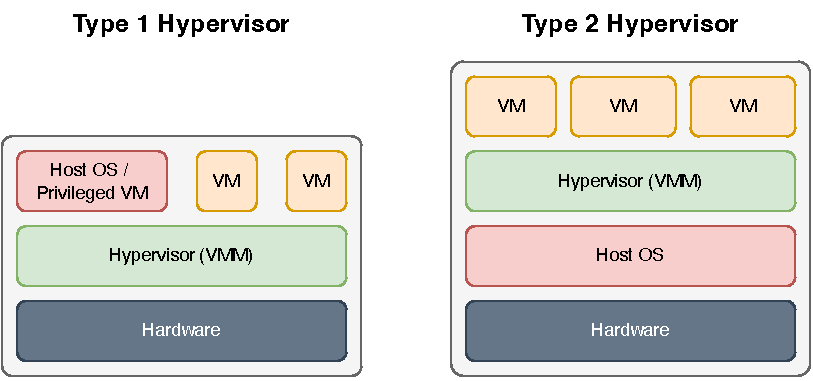
\includegraphics[width=0.7\textwidth]{img/hypervisors.pdf}
        \caption{Type 1 and Type 2 Hypervisors}
        \label{figure:hypervisors}
    \end{figure}

    \noindent Typically a distinction is made between two types of hypervisors as shown in \autoref{figure:hypervisors}. Type 1 hypervisors, also known as bare-metal hypervisors, lay directly on the hardware platform and create and run virtual machines directly on top of the hardware. This has the main benefit of offering high performance for VMs and is usually used for server systems where a high number of virtual servers is expected. In such systems, the VMs are typically centrally and remotely managed through APIs for efficient scaling capabilities. Since the hypervisor cannot rely on an underlying operating system, it has to tackle issues like managing drivers and file systems. In practice, this is often done by a trusted privileged VM that abstracts all of these challenges away for the other virtual machines. Compared to this, type 2 hypervisors which are also referred to as hosted hypervisors run on top of an operating system. This simplifies the responsibilities of the hypervisor, since the operating system already takes over the abstraction from the hardware and already has required system components like drivers. This approach however comes with the drawback of lower performance compared to type 1 hypervisors and is hence rather used for client systems, where the amount of VMs is very limited and simple UI-based management is usually enough. 
    
    When a virtualization technology is used for bare-metal machines in an IIoT platform the type 1 hypervisor should be chosen due to its high performance and API-based management, both of which allow for large-scale \cite{vs_anforderungsprofil}. \newline

    Now that we understand how virtualization works under the hood and how it should be used in an IIoT system, let us discuss why one would choose virtualization over plain bare-metal machines for provisioning (see \autoref{section:bare-metal-provisioning}). While using the hardware directly offers the best performance, using bare-metal machines still has certain drawbacks compared to a virtualized environment. Implementing multitenancy with robust isolation on bare-metal systems is challenging in contrast to simply using virtual machines, as it requires complex and often custom configurations to ensure both security and resource partitioning. This poses a problem when a single machine should be used by multiple parties that might affect each other, which could cause interference in the manufacturing/production site of an IIoT system (noisy neighbor problem). As already discovered in \autoref{section:bare-metal-provisioning} the biggest challenge however remains the lack of standardization when it comes to APIs for managing hardware directly. While there exist solutions (see \autoref{subsection:network-boot}) they are often based on outdated tools, dependent on the often very heterogeneous hardware, and are not robust due to many possible failures.\newline

    In contrast to this stands a hypervisor-based virtualized infrastructure, where each virtual machine is fully isolated from one another thus allowing for simple multipurpose usage of hardware. An example where this might be used is the deployment of a workload that cannot be containerized on a bare-metal server, which is already running Kubernetes. Using virtualization, this can easily be achieved by creating a separate isolated VM. Also, the fact that each virtual server is software-based offers enhanced infrastructure flexibility. Each server can be relocated to a different physical server effortlessly, created or destroyed on demand (``cattle not pets''), and vertically scaled by allocating more or fewer resources, among other features that expand the infrastructure's adaptability. The largest benefit however is the simple management of virtual servers through APIs. Commonly used virtualization platforms like VMware vSphere or ProxmoxVE offer rich APIs that feel similar to managing virtual machines within a cloud provider. These APIs can be used by ClusterAPI infrastructure providers directly (see \autoref{subsection:capi}) which is not only simpler but way more robust compared to the out-of-band management of bare-metal servers. Many multicluster management platforms (see \autoref{section:multicluster-mgmt}) like Rancher or Gardener that are capable of deploying Kubernetes onto a variety of infrastructure can also provision Kubernetes onto virtualization platforms directly. This way, a multicluster management solution can be used directly rather than building your own setup with ClusterAPI thus again reducing the system's complexity. 
    
    The use of virtualization on top of own hardware not only has benefits however. While with modern hardware, virtualization does not introduce much overhead anymore, the physical resources are still used a bit less efficiently due to the overhead of virtualization. Also, running a virtualization platform introduces more components and thus complexity that requires domain experts into the system. Lastly, production-ready virtualization platforms like VMware vSphere introduce additional cost, that needs to be accounted for \cite{baremetal_vs_hypervisor}. If a virtualization infrastructure already exists in the target environment however, it will simplify and robustify the provisioning mechanism immensely. \newline

    Overall, virtualization can significantly simplify the provisioning of bare-metal infrastructure for the edge and fog environments of the reference architecture described in \autoref{chapter:architecture-proposal}. Instructing ClusterAPI to interact with a virtualization platform can also improve the very crucial robustness of the infrastructure provisioning mechanism compared to using outdated out-of-band management solutions to provision hardware directly. Since drawbacks, i.e.\ cost, less efficient use of physical resources and additional complexity, exist as well, the decision whether to employ virtualization needs to be made dependent on the requirements of the project in question however.
        
        
    % \section{Security -- TODO: probably not really necessary as its not dealt with in this work}
    %     \begin{itemize}
    %         \item SigStore
    %         \item Golden images etc.
    %         \item Observability, Auditing
    %         \item Network Segregation
    %         \item RBAC / IAM
    %         \item Backups (3-2-1 Strategy) -- kein klassisches Security Thema
    %     \end{itemize}
        
    % \section{Solution patterns -- TODO: possibly a duplicate of 4.2}
    %     \begin{itemize}
    %         \item Where to use what?
    %         \item Pros / Cons of each 
    %     \end{itemize}